\documentclass{article}
\usepackage{enumerate}
\usepackage{amsmath}
\usepackage{amssymb}
\usepackage{graphicx}
\usepackage{subfigure}
\usepackage{geometry}
\usepackage{caption}
\usepackage{indentfirst}
\usepackage{fancyhdr}
\usepackage{ulem}
\usepackage{multirow}
\usepackage{tabu}
\usepackage{array}

\date{}
\pagestyle{fancy}
\fancyhead{}
\fancyhead[C]{
\includegraphics[width=\linewidth]{ji_header.png}}
\fancyfoot[C]{\thepage}
\renewcommand{\headrulewidth}{0pt}
\addtolength{\headheight}{4\baselineskip}
\geometry{top=4cm,bottom=4.0cm}
\begin{document}

\vspace*{3mm}

\begin{minipage}{0.6\linewidth}
\ 
\end{minipage}
\hfill
\begin{minipage}{0.38\linewidth}
\begin{center}
\huge\bfseries
Lab Report \\[8mm]
\fontsize{100pt}{\baselineskip}\selectfont
3
\end{center}
\end{minipage}

\vspace*{1cm}

{\huge\bfseries
\uline{UM-SJTU Joint Institute \phantom{xxxxxxxxxxxx}}
\vspace*{2mm}

Ve270 Introduction to Logic Design
}	

\vspace*{2cm}
\begin{center}
\LARGE
by \\[2mm]
\begin{tabular}{ll}
Liu Yihao & 515370910207 \\
Ma ShiYao & 515370910157
\end{tabular}

\vspace*{2cm}
Date: 2017-06-13
\end{center}

\vspace*{2cm}
\begin{center}
\Huge\bfseries
Design of a Simple ALU
\end{center}

\newpage

\section{Objectives}
To design a simple datapath using combinational building blocks in Xilinx ISE, and to implement the circuit in an FPGA chip.

\section{Problem Definition}
To form a Arithmetic and Logic Unit (ALU) which takes 4-bit input data and outputs the result(F and Cout). The algorithm being used is decided on the 2-input select signal. The algorithms are shown in Table \ref{def-table}.

\begin{table}[!hbtp]
\centering
\begin{tabular}{|c|c|c|c|c|}
\hline
S0 & S1 & F & Cout & Example \\\hline
0 & 0 & A$+$B & Carry out & A=1100, B=1110, F=1010, Cout=1 \\\hline
0 & 1 & A$-$B & Carry out & A=1100, B=1110, F=1110, Cout=0 \\\hline
1 & 0 & A and B & 0 & A=1100, B=1110, F=1100, Cout=0 \\\hline
1 & 1 & A or B & 0 & A=1100, B=1110, F=1110, Cout=0 \\\hline
\end{tabular}
\caption{Overall truth table}
\label{def-table}
\end{table}

\section{System Partitioning}
\begin{enumerate}
\item 8 Switches and 2 select signal buttons. Switches are used to input two 4-bit binary input A and B. The buttos are used to select the algorithm to be executed. Then the input signals will be transmitted to the inside circuit to calculate and come up with the result.
\item Inside circuit. To receive the input signals and get the result. It will outputs some signals that controls the LED to illuminate.
\item LED. LED is used as the output indicator. The illumination of different LED can indicate different different binary digit as the output F and Cout.
\end{enumerate}

\section{Design Entry}
The algorithm in this system was shown in Table \ref{algorithm-table}.

\begin{table}[!hbtp]
\centering
\begin{tabular}{|p{2cm}<{\centering}|p{2cm}<{\centering}|p{2cm}<{\centering}|p{2cm}<{\centering}|p{2cm}<{\centering}|}
\hline
\multicolumn{2}{|c|}{Select signal} & \multirow{2}{*}{Algorithm} & \multicolumn{2}{c|}{Output} \\\cline{1-2}\cline{4-5}
S0 & S1 & & F & Cout  \\\hline
0 & 0 & Add & A$+$B & Carry out  \\\hline
0 & 1 & Subtract & A$-$B & Carry out  \\\hline
1 & 0 & And & A and B & 0  \\\hline
1 & 1 & Or & A or B & 0  \\\hline
\end{tabular}
\caption{Algorithm table}
\label{algorithm-table}
\end{table}

According to the Table \ref{algorithm-table}, we designed the ALU circuit, shown in Figure \ref{design-alu}. \\

\begin{figure}[!htbp]
\centering
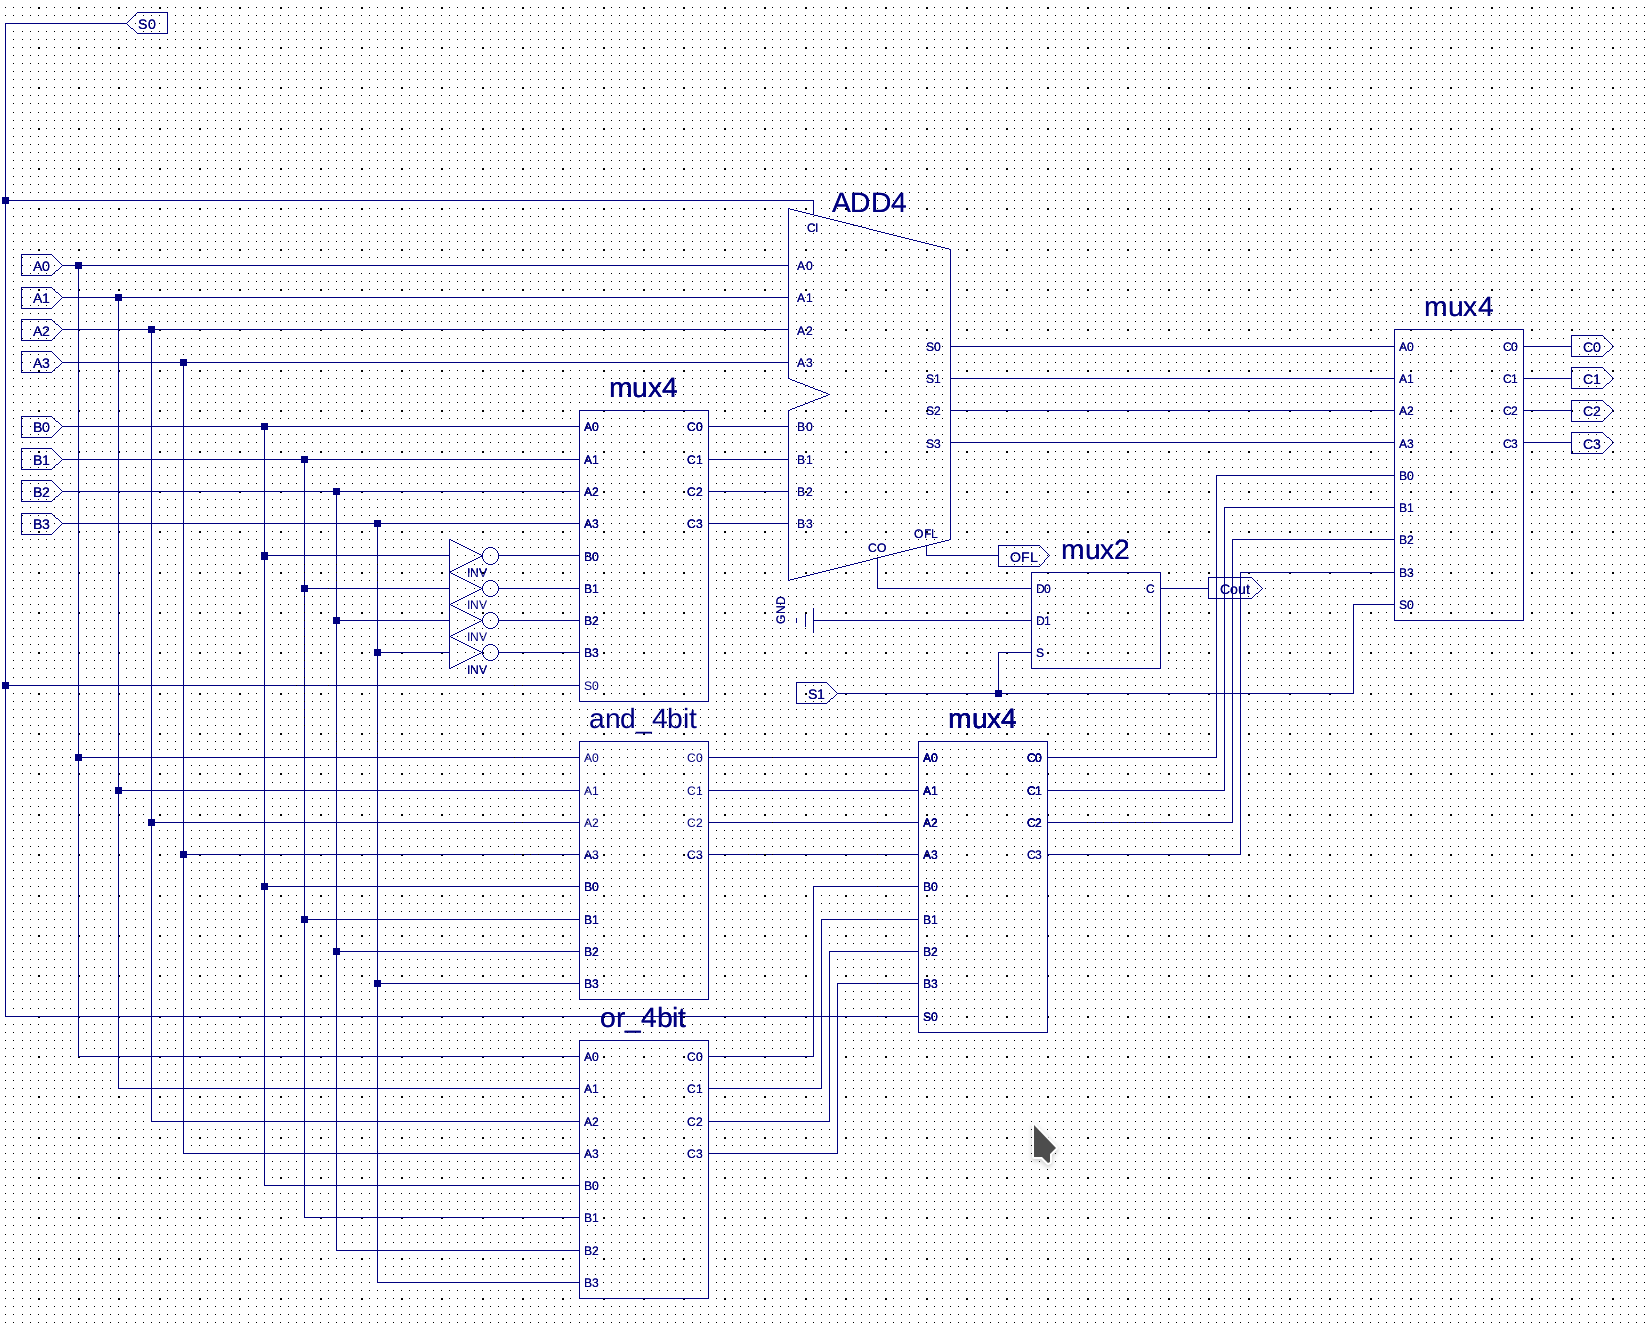
\includegraphics[width=0.8\linewidth]{alu.png}
\caption{Schematics design of ALU}
\label{design-alu}
\end{figure}

The inner design of several symbols were shown in Figure \ref{design-inner}. \\

\begin{figure}[!hbtp]
\centering
\subfigure[1 bit 2x1 mux]{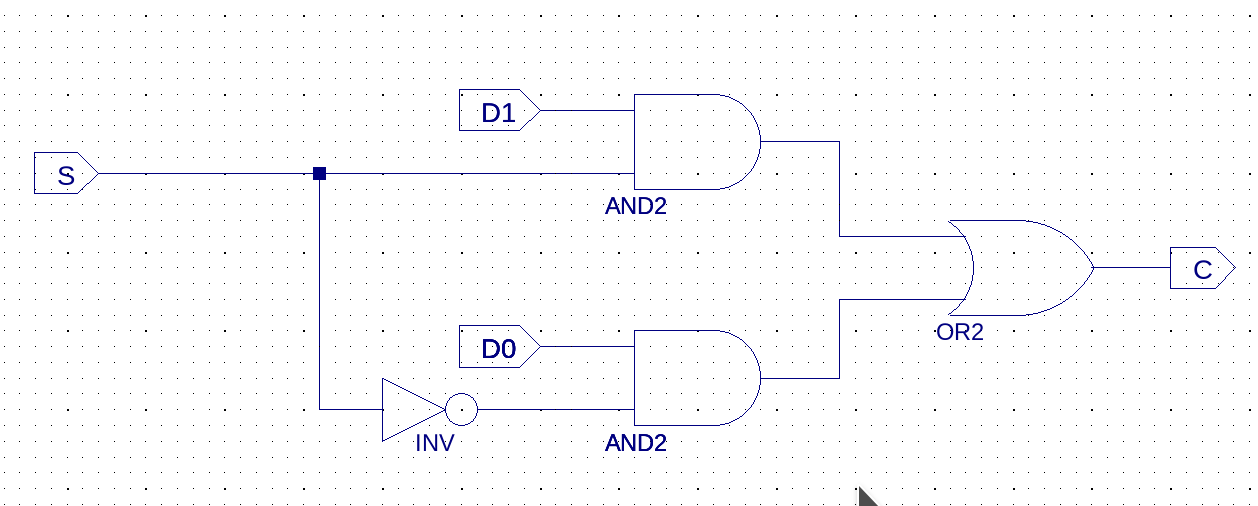
\includegraphics[width=0.5\linewidth]{mux2.png}}
\subfigure[8 bit 2x1 mux]{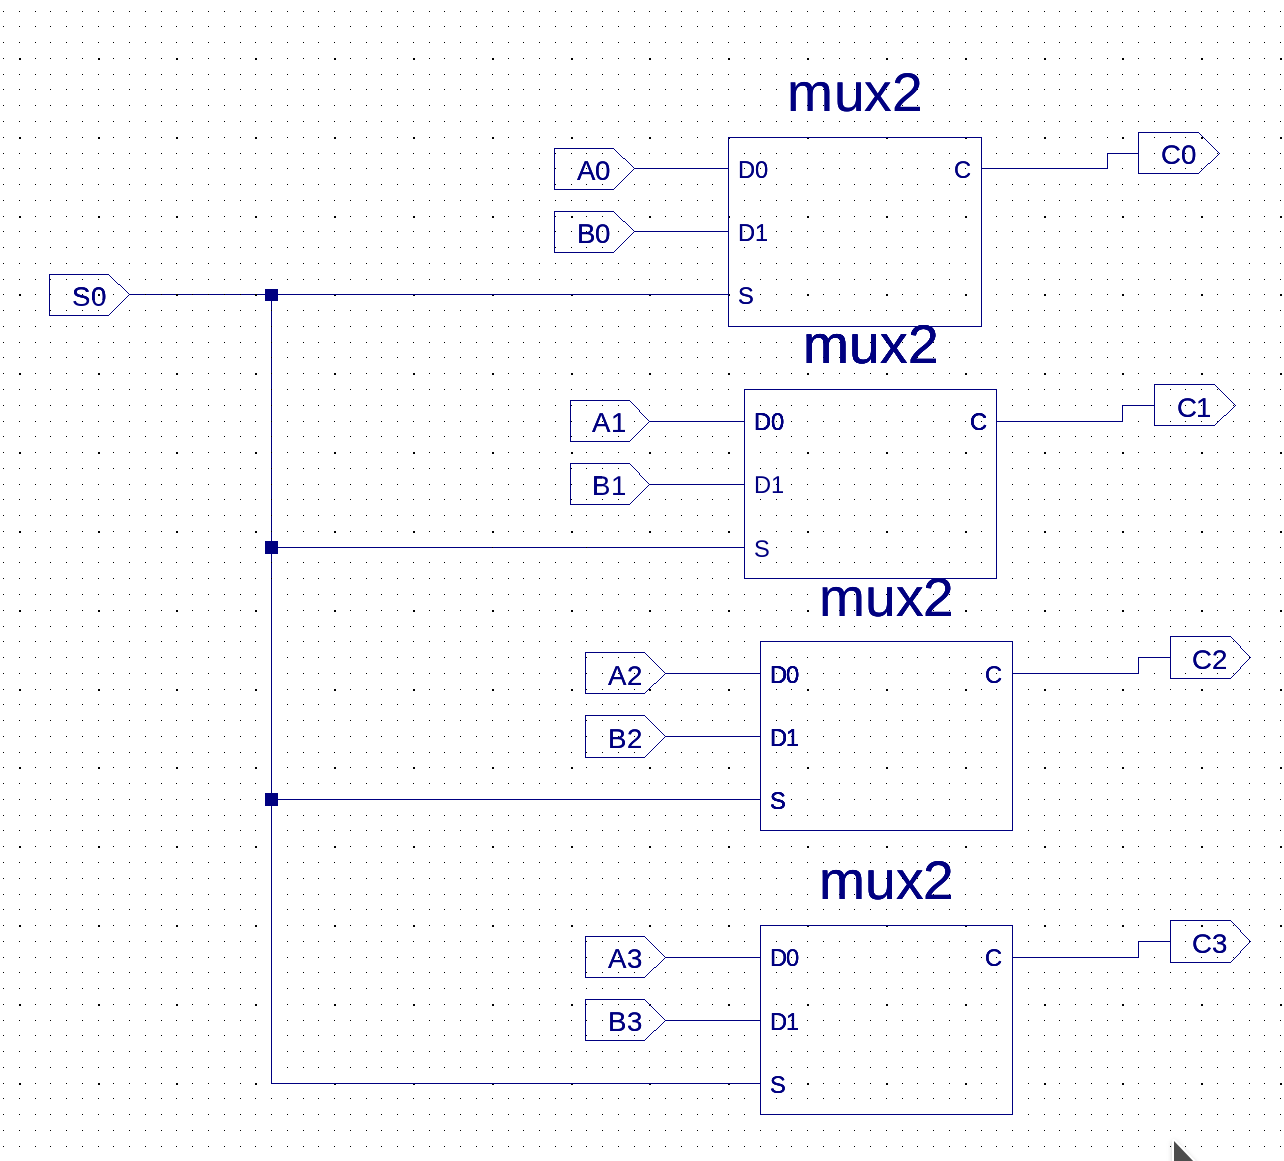
\includegraphics[width=0.45\linewidth]{mux4.png}}
\subfigure[8 bit and gate]{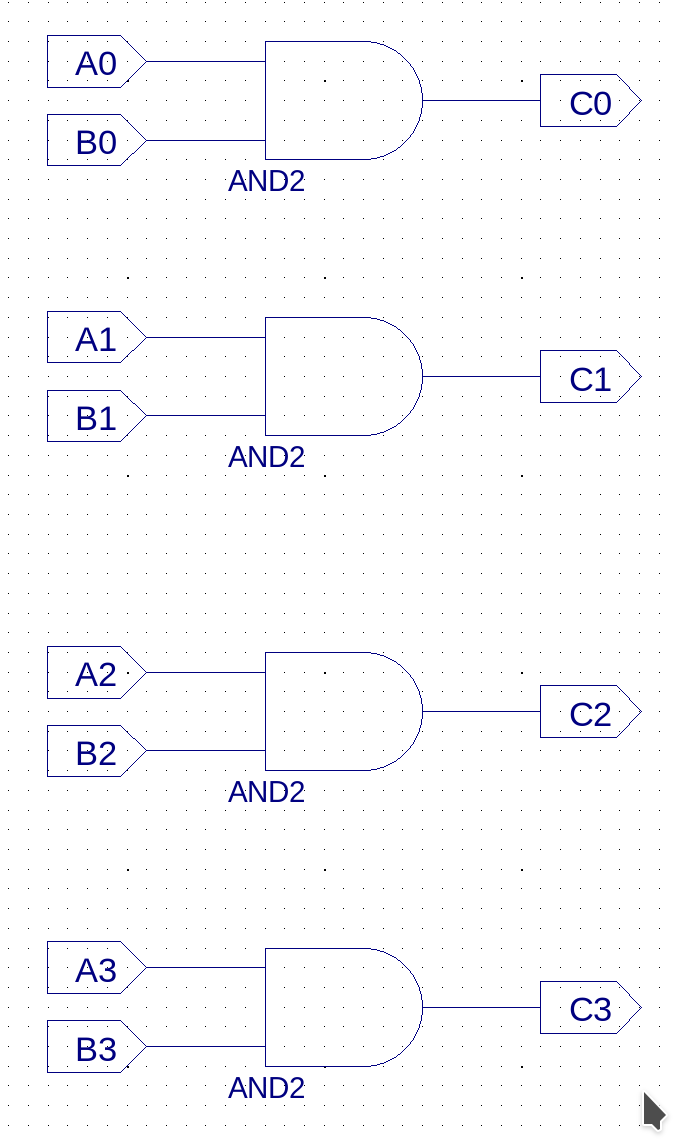
\includegraphics[width=0.4\linewidth]{and.png}}
\subfigure[8 bit or gate]{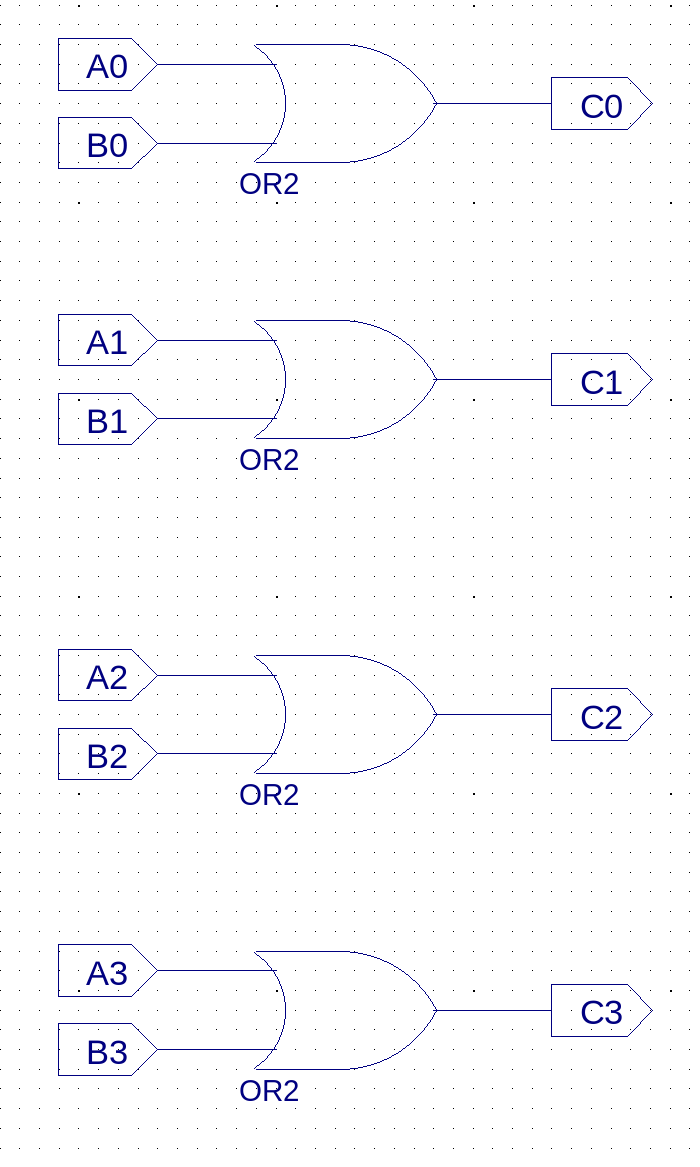
\includegraphics[width=0.4\linewidth]{or.png}}
\caption{Schematics design of symbols}
\label{design-inner}
\end{figure}

\newpage

\section{Test Plan}
\begin{center}
\begin{tabular}{|m{3cm}<{\centering}|m{10cm}|}
\hline
Test content & \multicolumn{1}{c|}{Test method} \\\hline
CA & \multirow{7}{10cm}{Input signal that needs corresponding LED segment to illuminate, then observe if it illuminates. If it illuminates when corresponding signal inputted, this subsystem passes the test; otherwise it fails.} \\\cline{1-1}
CB & \\\cline{1-1}
CC & \\\cline{1-1}
CD & \\\cline{1-1}
CE & \\\cline{1-1}
CF & \\\cline{1-1}
CG & \\\hline
The overall system & Input every kind of the 4-bit binary digit signal: 0001, 0010, 0011, 0100, 0101, 0110, 0111, 1000, 1001, then observe if LED displays the corresponding decimal digit:1,2,3,4,5,6,7,8,9. If so, the system passes the test; otherwise it fails. \\\hline
\end{tabular}
\end{center}

\section{Simulation Results}
We simulated the result of the overall system with input values in Table \ref{def-table}, shown in Figure \ref{simulation}.

\begin{figure}[!htbp]
\centering
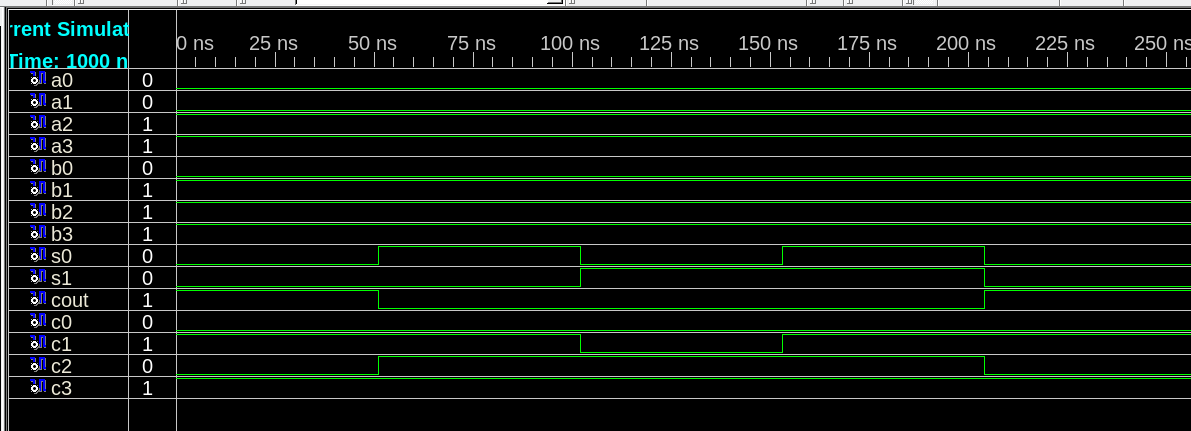
\includegraphics[width=0.9\linewidth]{simulation.png}
\caption{Simulation of ALU}
\label{simulation}
\end{figure}

We found the values in the simulation identical to Table \ref{def-table}.


\newpage

\section{Conclusion}
In this lab, we successfully finished it finally, but we also met with some problems in the process. Some existing modules in ISE will cause error in the simulation and pace process, such as the inverse-4 and mux-4, so we have to build a new module ourselves. We practiced build a ALU with 2-bit select input signal and four kinds of  algorithms.

\section{Appendix}
The schematics of our design had been submitted to canvas before.


\end{document}